\hqlabel{subsubsection: Test-and-Set based lock}{\subsubsection{Test-and-Set based lock}}

The \definition{Test-and-Set instruction} is a fundamental \textbf{atomic operation used for synchronization} in multiprocessor systems. It \textbf{checks the value of a lock variable and sets it to a new value in one uninterruptible action}. The operation ensures that no other processors can modify the lock variable simultaneously, preventing race conditions.

\highspace
\begin{flushleft}
    \textcolor{Green3}{\faIcon{question-circle} \textbf{How does it work?}}
\end{flushleft}
It performs \textbf{two actions in one \underline{uninterruptible step}}:
\begin{enumerate}
    \item It loads the value from a memory address into a register;
    \item Then sets the memory address to a specified value (usually indicating the lock is acquired).
\end{enumerate}
\begin{lstlisting}
ts R0, mem[addr]    // load mem[addr] into R0
                    // if mem[addr] is 0, set mem[addr] to 1
\end{lstlisting}

\highspace
\begin{flushleft}
    \textcolor{Green3}{\faIcon{lock} \textbf{Lock Implementation}}
\end{flushleft}
To implement a lock using the test-and-set instruction, we must \textbf{repeatedly attempt to acquire the lock until it is free}.
\begin{lstlisting}[mathescape=true]
lock:   
    ts  R0, mem[addr]   // Attempt to acquire the lock
    bnz R0, lock        // If the lock was not free (R0 $\ne$ 0),
                        // retry
\end{lstlisting}
\begin{itemize}
    \item \texttt{ts R0, mem[addr]}: Atomically loads the value at \texttt{mem[addr]} into register \texttt{R0} and sets \texttt{mem[addr]} to \texttt{1} if it was \texttt{0}.

    \item \texttt{bnz R0, lock}: If \texttt{R0} is non-zero (meaning the lock was already held), it branches back to the start and retries.
\end{itemize}

\highspace
\begin{flushleft}
    \textcolor{Green3}{\faIcon{lock-open} \textbf{Unlock Implementation}}
\end{flushleft}
To release the lock, simply we \textbf{set the lock variable back to \texttt{0}}.
\begin{lstlisting}
unlock: 
    st  mem[addr], #0    // Release the lock by storing 0
\end{lstlisting}
\begin{itemize}
    \item \texttt{st mem[addr], \#0}: Stores \texttt{0} at the memory address \texttt{addr}, indicating the lock is now free.
\end{itemize}

\newpage

\begin{flushleft}
    \textcolor{Red2}{\faIcon{exclamation-triangle} \textbf{Coherence Protocol}}
\end{flushleft}
Using test-and-set based locking is fundamental to \textbf{maintaining consistency across multiple processor caches by ensuring that all processors have the same view of the lock variable}. So it involves invalidating and updating cache lines across processors as the lock state changes.
\begin{figure}[!htp]
    \centering
    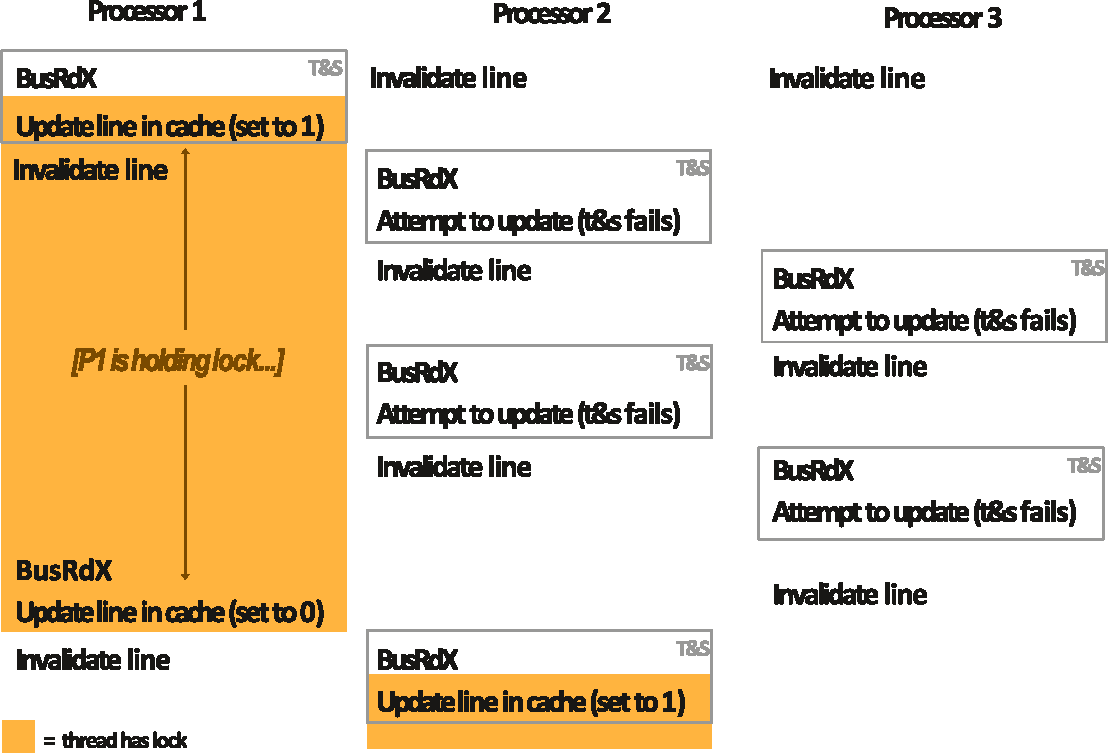
\includegraphics[width=\textwidth]{img/test-and-set-1.pdf}
\end{figure}
\begin{itemize}
    \item Processor 1 (\texttt{P1}):
    \begin{itemize}
        \item \important{Acquiring Lock}:
        \begin{itemize}
            \item \textbf{BusRdX Request}: \texttt{P1} sends a Bus Read Exclusive (\texttt{BusRdX}) request to acquire the lock.
            \item \textbf{Cache Update}: \texttt{P1} sets the lock value to 1 in its cache, indicating the lock is held.
            \item \textbf{Invalidation}: Other processors' caches are invalidated for the lock variable.
        \end{itemize}

        \item \important{Releasing Lock}:
        \begin{itemize}
            \item \textbf{BusRdX Request}: \texttt{P1} sends another \texttt{BusRdX} request to release the lock.
            \item \textbf{Cache Update}: \texttt{P1} sets the lock value to 0 in its cache, indicating the lock is free.
            \item \textbf{Invalidation}: Other processors' caches are invalidated for the lock variable.
        \end{itemize}
    \end{itemize}

    \newpage
    
    \item Processor 2 (\texttt{P2}) and Processor 3 (\texttt{P3}):
    \begin{itemize}
        \item \important{Attempting to Acquire Lock}:
        \begin{itemize}
            \item \textbf{Invalidation}: Their cache lines for the lock are initially invalidated.
            \item \textbf{BusRdX Request}: Both processors send \texttt{BusRdX} requests to acquire the lock.
            \item \textbf{Retry Loop}: If the lock is not free, they continuously retry, causing repeated \texttt{BusRdX} requests.
        \end{itemize}
    \end{itemize}
\end{itemize}

\highspace
\begin{flushleft}
    \textcolor{Green3}{\faIcon{question-circle} \textbf{Implications of Coherence Traffic}}
\end{flushleft}
\begin{itemize}
    \item \important{Contention}. \textbf{High contention occurs when multiple processors compete for the same lock at the same time}.
    
    Each processor continuously attempts to execute the test-and-set instruction, resulting in repeated \texttt{BusRdX} requests. This competition \textbf{generates significant traffic on the memory bus and forces processors to repeatedly invalidate each other's cache lines for the lock variable}.
    
    The result is a high level of contention that can \textbf{cause delays and inefficiencies as processors wait for the lock to become available}.


    \item \important{Performance Impact}. \textbf{The frequent \texttt{BusRdX} requests and resulting cache invalidations can significantly degrade system performance}, \textbf{especially as the number of processors increases}.
    
    Each \texttt{BusRdX} request incurs a cost in terms of memory bus usage and latency. As more processors contend for the lock, the cumulative effect of these requests becomes more pronounced, leading to:
    \begin{itemize}
        \item[\textcolor{Red2}{\faIcon{times}}] \textcolor{Red2}{\textbf{Increased Latency}}: The time taken for processors to acquire and release the lock increases, slowing down the overall execution of the program.
        
        \item[\textcolor{Red2}{\faIcon{times}}] \textcolor{Red2}{\textbf{Memory Bus Saturation}}: The memory bus becomes saturated with coherence traffic, reducing the available bandwidth for other memory operations.
        
        \item[\textcolor{Red2}{\faIcon{times}}] \textcolor{Red2}{\textbf{Inefficiency}}: Processors spend more time waiting and retrying to acquire the lock, leading to inefficient use of processing resources.
    \end{itemize}
\end{itemize}

\newpage

\begin{flushleft}
    \textcolor{Green3}{\faIcon{tachometer-alt} \textbf{Test-and-Set Performance}}
\end{flushleft}
The following graph plots the performance of the test-and-set lock in terms of time (in microseconds) versus the number of processors. It specifically measures the time taken to acquire and release the lock as the number of processors increases.
\begin{figure}[!htp]
    \centering
    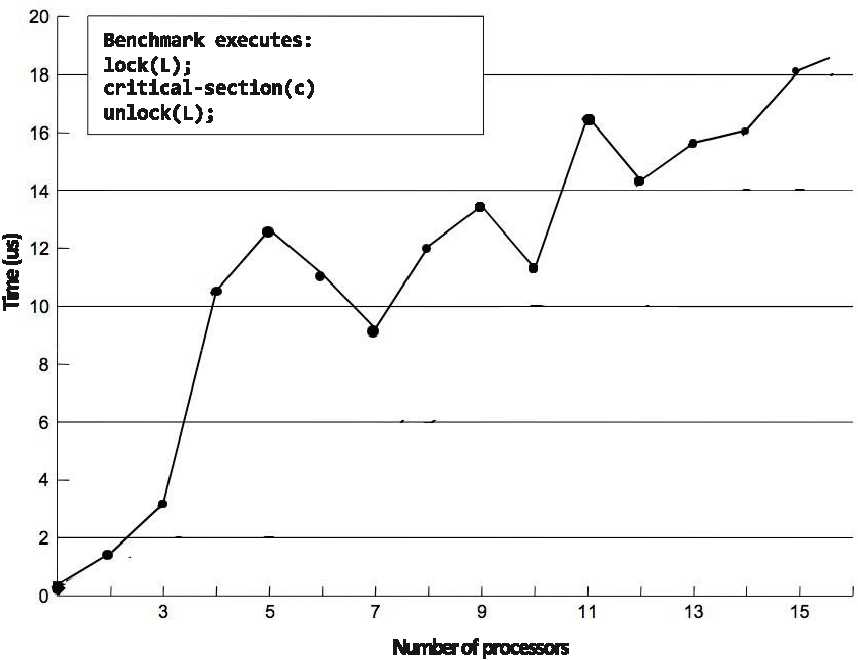
\includegraphics[width=\textwidth]{img/test-and-set-performance-1.pdf}
\end{figure}
\begin{itemize}
    \item \texttt{X-Axis}: Number of processors (ranging from 0 to 16).
    
    \item \texttt{Y-Axis}: Time in microseconds (ranging from 0 to 20).
    
    \item \textbf{Initial Increase}: As the number of processors increases from 1 to 4, the time taken to acquire and release the lock increases significantly.
    
    \item \textbf{Fluctuations}: There is a noticeable dip in time around 7 processors, followed by fluctuations as the number of processors continues to increase.
    
    \item \textbf{Overall Trend}: Despite the fluctuations, the \textbf{general trend shows an upward increase in time with more processors}, indicating \textbf{higher contention}.
\end{itemize}
The performance of the test-and-set lock shows that with an \textbf{increasing number of processors}, the \textbf{time to acquire and release the lock increases due to contention and coherence traffic}.